\section{Experiments}
\label{sec:experiments}

\subsection{Experimental Setup}

\subsubsection{Evaluation Questions}
\label{subsubsec:evaluation_questions}
The evaluation addresses five questions:
\begin{itemize}
    \item \textbf{RQ1: Rule-space expansion.} How many distinct rule candidates do the two generation strategies contribute?
    \item \textbf{RQ2: Executable detection.} Do the final rule families detect complementary defects on RuleTest-94?
    \item \textbf{RQ3: Adaptive optimization.} Does a learned policy outperform fixed and sequential schedules under identical graph transitions and budgets?
    \item \textbf{RQ4: Constraint checking.} What does generated validation add beyond structural SHACL-style checks?
    \item \textbf{RQ5: End-to-end robustness.} Does the quality-control layer improve deterministic and API-extracted KGs?
\end{itemize}

\subsubsection{Evaluation Pools and Scope}
\label{subsubsec:testset}
RuleTest-94 is a designed executable test suite, not a prevalence sample. It contains 30 clean cases and 64 defective cases: 10 hierarchy reversals, 10 absurd relations, 10 reversed-supervision relations, 30 procedural or missing-field defects, and 4 specialist constraints. The clean cases support false-positive measurement. Each detector writes a prediction for every case, allowing the confusion matrices to be reconstructed from the released CSV files.

The candidate-level experiment replays 9,456 successful stored generation responses: 4,728 deletion-completion calls and 4,728 augmentation-expansion calls. Its unit is a canonicalized candidate rule, so candidate counts must not be interpreted as detection accuracy. The RL benchmark uses a separate 450-document TNEWS/CLUE graph with controlled graph mutations. The deterministic external benchmark uses 3,000 documents, and the API extraction benchmark uses 45 titles. Keeping these pools separate prevents the designed RuleTest suite or controlled corruption manifest from being presented as naturally occurring test data.

\subsubsection{Runtime and Reproducibility Settings}
\label{subsubsec:runtime_reproducibility}
All deterministic scripts use fixed recorded seeds. The RL comparison uses ten paired evaluation seeds and ten independently trained models per learned method. It archives checkpoints, all evaluation transitions, and per-episode histories. The API benchmark makes 45 calls to Qwen3.8-27B-no-thinking through the configured OpenAI-compatible endpoint with proxy inheritance disabled; parse or request failures remain in the denominator. Rule candidates are materialized through the validation pipeline in Section~\ref{subsubsec:rule_materialization}.

\subsection{Rule Generation Results}
% 放到4.3
\subsubsection{Quantity Comparison}

\begin{table}[t]
    \centering
    \caption{Comparison of Rule Generation Quantity}
    \label{tab:rule_quantity}
    \footnotesize
    \setlength{\tabcolsep}{2pt}
    \begin{tabular*}{\columnwidth}{@{\extracolsep{\fill}}l c c c@{}}
    \toprule
    Rule Type & Expert & Auto-gen. & Improv. \\
    \midrule
    Entity type & 7 & 77 & 11.00$\times$ \\
    Relation type & 9 & 80 & 8.89$\times$ \\
    Other type constraints & 21 & 15 & 0.71$\times$ \\
    Hierarchical & 0 & 31 & Exclusive \\
    Procedural & 0 & 88 & Exclusive \\
    Total & 37 & 291 & 7.86$\times$ \\
    \bottomrule
    \end{tabular*}
\end{table}

\begin{figure*}[t]
    \centering
    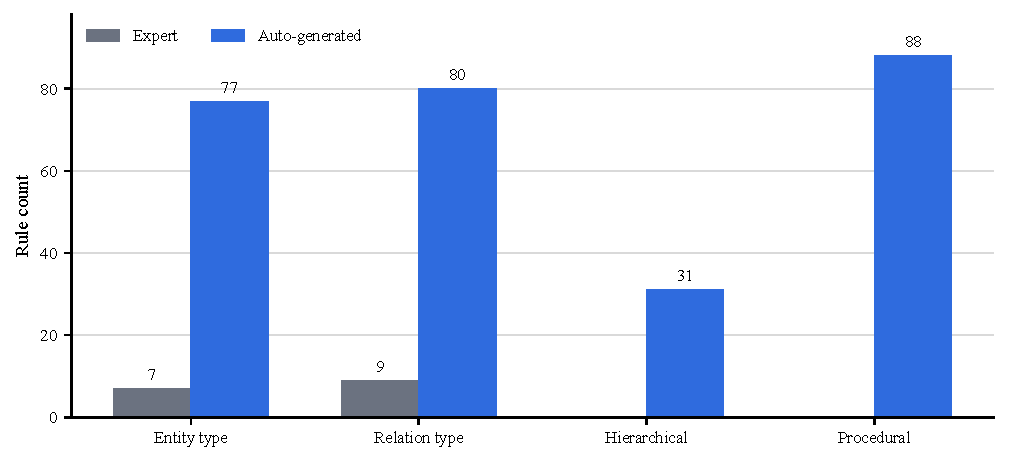
\includegraphics[width=0.95\textwidth]{figure/experiments/rule_quantity.pdf}
    \caption{Comparison of Rule Generation Quantity}
    \label{fig:rule_quantity}
\end{figure*}

\textbf{Key Finding:} The evaluated generated set contains 291 rules versus 37 expert rules (7.86$\times$), including 31 hierarchical and 88 procedural rules absent from the expert set.

\subsubsection{Executable Detection on RuleTest-94}

\begin{table}[t]
    \centering
    \caption{Executable rule detection on RuleTest-94.}
    \label{tab:rule_performance}
    \begin{tabular}{l c c c c}
    \toprule
    Rule set & Precision & Recall & F1 & Family cov. \\
    \midrule
    Expert structural & 1.000 & 0.469 & 0.638 & 0.600 \\
    \textbf{System union} & \textbf{1.000} & \textbf{1.000} & \textbf{1.000} & \textbf{1.000} \\
    \bottomrule
    \end{tabular}
\end{table}

The expert structural detector identifies 30 of 64 defects and makes no false-positive prediction on the 30 clean cases. The system union identifies all 64 defects with no false positives on this designed suite. Its additional 34 detections are procedural, missing-field, or specialist cases, so its unique detection capability relative to the expert detector is $34/64=0.531$. The 95\% Wilson interval for system precision uses 64 predicted positives and is $[0.943,1.000]$. These values establish executable suite coverage; they do not imply perfect open-world precision.

\subsubsection{Candidate-Level Dual-Strategy Ablation}
\label{subsubsec:dual_strategy_ablation}

To verify that deletion completion and augmentation expansion contribute complementary rule candidates, we re-aggregate the stored LLM outputs by strategy before final validation and deduplication. This analysis does not replace executable detection on RuleTest-94; it measures how much of the candidate rule space each strategy contributes.

\begin{table}[t]
    \centering
    \caption{Candidate-level ablation of deletion and augmentation strategies on stored government-domain generation logs.}
    \label{tab:dual_strategy_candidate_ablation}
    \footnotesize
    \setlength{\tabcolsep}{2pt}
    \begin{tabular*}{\columnwidth}{@{\extracolsep{\fill}}l c c c c@{}}
    \toprule
    Strategy & Calls & Cand. Rules & Cov. vs Dual & Unique \\
    \midrule
    Deletion only & 20 & 285 & 0.483 & 262 \\
    Augmentation only & 20 & 328 & 0.556 & 305 \\
    \textbf{Dual strategy} & \textbf{40} & \textbf{590} & \textbf{1.000} & \textbf{567} \\
    \bottomrule
    \end{tabular*}
\end{table}

The two strategies overlap on only 23 candidate rules in this controlled 20-item log, while deletion contributes 262 unique candidates and augmentation contributes 305. The dual strategy therefore yields 79.9\% more candidates than the stronger single strategy. Running the same aggregation on the full available government-domain log (4,728 items per strategy) gives the same pattern: deletion produces 32,955 candidates, augmentation produces 41,683, and the dual strategy produces 71,656 candidates, a 71.9\% gain over the stronger single strategy. This supports the complementarity claim at the generation stage; final rule precision still depends on the validation and filtering pipeline described in Section~\ref{subsubsec:rule_materialization}.

\subsubsection{Rule-Family Final Ablation on RuleTest-94}
\label{subsubsec:rule_family_final_ablation}

The candidate-level ablation above measures generated rule diversity before final validation. To test whether the two strategy families also provide complementary executable detection coverage, we run a deterministic rule-family ablation on RuleTest-94. Deletion-family rules cover procedural, missing-field, and specialist constraints, while augmentation-family rules cover structural relation, hierarchy, and type-direction constraints. This experiment should be interpreted as a final \emph{rule-family} ablation, not as per-rule provenance labeling for every generated LLM rule.

\begin{table}[t]
    \centering
    \caption{Rule-family final ablation on RuleTest-94.}
    \label{tab:rule_family_final_ablation}
    \footnotesize
    \setlength{\tabcolsep}{2pt}
    \begin{tabular*}{\columnwidth}{@{\extracolsep{\fill}}l c c c c@{}}
    \toprule
    Strategy & Precision & Recall & F1 & Fam. Cov. \\
    \midrule
    Deletion-family only & 1.000 & 0.531 & 0.694 & 0.400 \\
    Augmentation-family only & 1.000 & 0.469 & 0.638 & 0.600 \\
    \textbf{Dual strategy} & \textbf{1.000} & \textbf{1.000} & \textbf{1.000} & \textbf{1.000} \\
    \bottomrule
    \end{tabular*}
\end{table}

The deletion-family detector captures 34 of 64 defective cases, while the augmentation-family detector captures a different set of 30 structural cases. Their union detects all 64 defective cases without false positives on the 30 clean cases in RuleTest-94. This result strengthens the complementarity claim: the two strategies are not merely producing more candidates, but cover different executable defect families.
We use this result as supporting evidence for strategy complementarity; the detection comparison remains the executable RuleTest-94 evaluation in Table~\ref{tab:rule_performance}.

\subsection{RL Co-optimization on Executable Graph Transitions}
\label{subsec:rl_results}

\subsubsection{Controlled Environment and Protocol}
The policy benchmark uses 450 balanced TNEWS/CLUE documents (30 from each of 15 categories) to construct a clean graph with 873 nodes and 1,083 relations. For each evaluation seed, the environment injects seed-dependent amounts of four defects: isolated nodes, exact duplicate relations, schema-invalid relations, and dangling edges. Online rule metrics use a fixed 180-case validation inventory containing 30 positives for each defect family and 60 clean cases; the four valid modules each detect 27 of 30 family positives plus two clean cases, while three low-precision modules exercise the pruning action. This inventory is part of the controlled environment and is separate from RuleTest-94. Each action changes the graph or active rule set, after which all four graph metrics and three rule metrics are recomputed. The policy cannot observe the corruption manifest. Relation restoration consults the manifest only after the invalid-relation validator has fired, analogous to using a trusted source record for repair.

We train standard DQN and Double DQN independently for ten seeds, using 250 episodes per seed. Evaluation uses the same ten paired scenario seeds for every method. Besides random selection, we implement graph-only, rule-only, alternating, rule-first-then-fix, and fix-first-then-rule schedules. A one-step myopic policy clones the current environment and executes every feasible action before choosing; because this gives it a transition model unavailable to the other methods, we report it as a model-informed upper-bound diagnostic rather than as the primary baseline. Normalized joint quality is
\begin{equation}
\bar Q=\frac{Q(G)+0.4Q_{\mathrm{online}}(R)}{1.4},
\end{equation}
and AUC is the mean of $\bar Q$ over the decision trajectory. Convergence is the first step at which $\bar Q\geq0.98$; a value of 19 denotes failure within the 18-step budget.

\subsubsection{Policy Comparison}
\begin{table*}[t]
\centering
\caption{Co-optimization results on executable graph transitions (mean $\pm$ standard deviation over 10 paired seeds).}
\label{tab:rl_ablation}
\small
\setlength{\tabcolsep}{4pt}
\begin{tabular}{l c c c c c}
\toprule
Policy & Final $\bar Q$ & Trajectory AUC & Steps to 0.98 & Calls & Edits \\
\midrule
Random & $0.9535\pm0.0266$ & $0.8829\pm0.0318$ & 19.0 & 8.3 & 151.4 \\
Enhancement only & $0.6785\pm0.0036$ & $0.6785\pm0.0036$ & 19.0 & 0.0 & 0.0 \\
Rule only & $0.9373\pm0.0036$ & $0.9225\pm0.0036$ & 19.0 & 18.0 & 24.0 \\
Alternating & $0.9634\pm0.0007$ & $0.9261\pm0.0020$ & 19.0 & 12.0 & 215.0 \\
Rule first, then fix & $0.9747\pm0.0004$ & $0.9365\pm0.0024$ & 19.0 & 8.0 & 232.7 \\
Fix first, then rule & $0.9330\pm0.0036$ & $0.8204\pm0.0036$ & 19.0 & 12.0 & 13.0 \\
Myopic model-informed & $\mathbf{0.9825}\pm\mathbf{0.0001}$ & $\mathbf{0.9576}\pm\mathbf{0.0009}$ & $\mathbf{13.2}$ & 4.0 & 242.2 \\
DQN & $0.9813\pm0.0017$ & $0.9530\pm0.0041$ & 16.8 & 4.1 & 233.8 \\
\textbf{Double DQN} & $\mathbf{0.9812}\pm\mathbf{0.0013}$ & $\mathbf{0.9531}\pm\mathbf{0.0021}$ & $\mathbf{17.0}$ & \textbf{4.0} & 234.9 \\
\bottomrule
\end{tabular}
\end{table*}

Double DQN improves final quality by 0.0065 and AUC by 0.0166 over the strongest non-oracle fixed schedule, rule-first-then-fix. Across the ten paired seeds, the 95\% paired-bootstrap intervals are $[0.0058,0.0071]$ for final quality and $[0.0156,0.0178]$ for AUC; both one-sided Wilcoxon tests give $p=0.000977$. The learned policy also reduces rule-generation calls from 8.0 to 4.0. DQN and Double DQN have essentially the same mean performance; Double DQN has lower AUC variability ($0.0021$ versus $0.0041$). We therefore attribute the gain to learned state-conditioned control and do not claim a significant mean advantage of Double DQN over standard DQN.

The myopic model-informed policy remains slightly stronger in AUC. This is expected because it evaluates every one-step transition before acting. Double DQN approaches that upper bound without access to the transition function: its final-quality gap is 0.0013 and its AUC gap is 0.0045.

\begin{figure}[t]
\centering
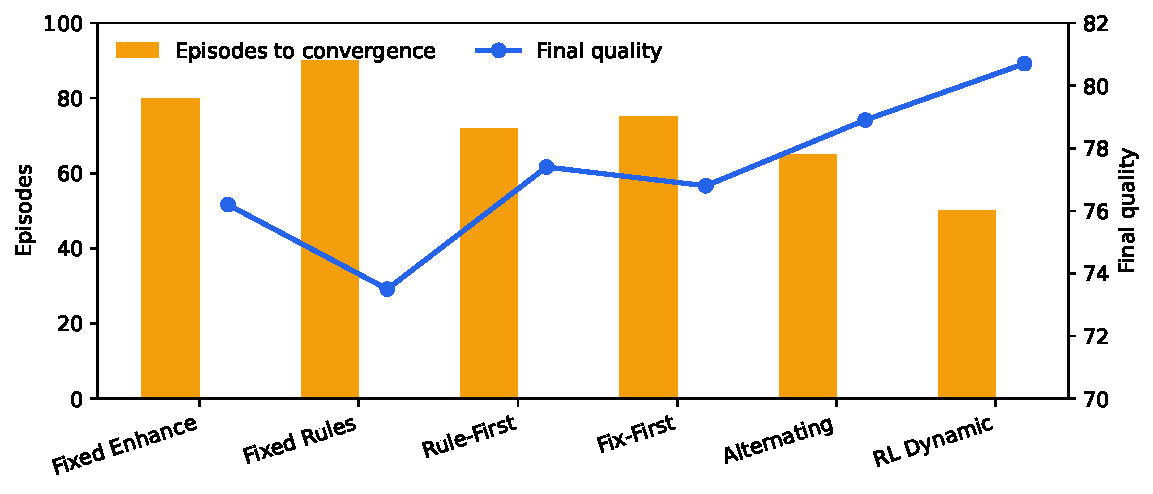
\includegraphics[width=\columnwidth]{figure/experiments/rl_convergence.pdf}
\caption{Evaluation trajectories over ten paired seeds. Lines show means and shaded bands show one standard deviation. The myopic curve is a model-informed upper bound.}
\label{fig:rl_convergence}
\end{figure}

\subsubsection{Learned Action Use and Reproducibility}
The Double DQN policy selects mixed rule generation exactly twice per run on average, activating the four high-precision validators with four accounted calls. It then allocates the remaining decisions according to the unresolved violation counts: 3.3 isolation cleanups, 5.2 deduplication steps, 4.0 relation repairs, and 3.5 dangling-edge cleanups per run. This ordering is state-dependent because corruption rates differ by seed. It does not repeatedly call the rule generator after all four validators are available.

The experiment archives 2,500 training episodes per learned method, 1,616 evaluation transitions across all policies, twenty model checkpoints, per-seed metrics, and the exact statistical test inputs. Training makes no API calls. The stored dual-strategy generation log contains 9,456 successful calls (4,728 per strategy), which are reused for the separate rule-content analyses rather than regenerated inside RL episodes.


\subsection{Comparison with Constraint-Checking Baseline}
\label{subsec:shacl_baseline}

We compare with a deterministic constraint-checking baseline implemented with SHACL-style RDF validation. This baseline receives deduplicated RDF triples and checks schema-conformance constraints, but it does not access the source text, LLM prompts, or generated procedural/value rules. The experiment therefore measures whether conventional graph-shape validation is sufficient for our quality-control task.

\begin{table}[t]
    \centering
    \caption{SHACL-style structural validation baseline on three domains.}
    \label{tab:shacl_baseline}
    \footnotesize
    \setlength{\tabcolsep}{2pt}
    \begin{tabular*}{\columnwidth}{@{\extracolsep{\fill}}l r r c c@{}}
    \toprule
    Domain & Raw Triples & RDF Dedup. & Removed & $Q$ \\
    \midrule
    Gov. Affairs & 13,892 & 10,771 & 0 & 79.87 \\
    Finance & 2,264 & 539 & 0 & 70.42 \\
    Env. & 2,345 & 378 & 0 & 65.25 \\
    \midrule
    Average & 6,167 & 3,896 & 0 & 71.85 \\
    \bottomrule
    \end{tabular*}
\end{table}

The SHACL-style baseline conforms after RDF deduplication and removes no additional triples, because its schema-level constraints cannot express many of the source-text-dependent, value-range, temporal, and procedural defects targeted by our rule set. Its average quality score is 71.85, limited by redundancy, semantic soundness, and residual logical checks rather than SHACL conformance. This supports the need for generated domain rules beyond static shape validation.

\subsection{External Benchmark Platform}
\label{subsec:external_benchmark}

To test whether the quality-enhancement pipeline behaves robustly outside the three in-domain regulatory datasets, we built a local end-to-end benchmark platform using two existing benchmark-style resources in the repository. First, we use a TNEWS/CLUE-style Chinese news dataset as an out-of-domain text source. A deterministic extractor constructs a document--category--entity KG from 3,000 balanced news titles across 15 categories; we then inject duplicate triples, invalid relations, and isolated nodes, and run the local repair pipeline. Second, we use the 94-case rule-test set as a labeled rule-detection benchmark. This benchmark is fully local and makes no LLM/API calls, so it evaluates KG quality control and rule execution rather than LLM extraction quality.

\begin{table}[t]
    \centering
    \caption{TNEWS/CLUE local end-to-end KG quality benchmark.}
    \label{tab:tnews_external_benchmark}
    \footnotesize
    \setlength{\tabcolsep}{2pt}
    \begin{tabular*}{\columnwidth}{@{\extracolsep{\fill}}l c c c c@{}}
    \toprule
    Stage & Nodes & Relations & Invalid & $Q$ \\
    \midrule
    Clean extraction & 10,871 & 20,827 & 0.000 & 99.89 \\
    Corrupted KG & 11,414 & 22,909 & 0.050 & 94.93 \\
    Repaired KG & 10,822 & 19,799 & 0.000 & 100.00 \\
    \bottomrule
    \end{tabular*}
\end{table}

The repair pipeline removes injected invalid relations, duplicate triples, and isolated noise nodes, improving $Q$ from 94.93 to 100.00 and recovering the full injected quality gap under this deterministic benchmark. The full report is generated by \texttt{exps/external\_benchmark\_runner.py}.

\begin{table}[t]
    \centering
    \caption{RuleTest-94 local rule-detection benchmark.}
    \label{tab:ruletest_external_benchmark}
    \footnotesize
    \setlength{\tabcolsep}{2pt}
    \begin{tabular*}{\columnwidth}{@{\extracolsep{\fill}}l c c c c@{}}
    \toprule
    Detector & Precision & Recall & F1 & Accuracy \\
    \midrule
    Expert structural rules & 1.000 & 0.469 & 0.638 & 0.638 \\
    System rule detector & 1.000 & 1.000 & 1.000 & 1.000 \\
    \bottomrule
    \end{tabular*}
\end{table}

The expert structural baseline detects hierarchy reversal, absurd relations, and reversed supervision, but misses procedural, missing-field, and specialist-rule defects. The system rule detector covers these additional categories and passes all 64 defective cases in RuleTest-94 without false positives. Because RuleTest-94 is a designed local test suite, this result should be interpreted as benchmark-suite coverage rather than universal real-world precision.

\subsection{API-Backed LLM Extraction Benchmark}
\label{subsec:api_llm_benchmark}

The local TNEWS/CLUE benchmark above isolates the quality-control layer under deterministic extraction. To additionally test the full extraction path, we run an API-backed LLM extraction benchmark on 45 TNEWS/CLUE titles covering 15 categories. The model is Qwen3.8-27B-no-thinking. TNEWS category labels are used as silver labels for category inference, and provided title keywords are used as weak silver mentions for entity coverage. This is not a gold triple-level benchmark; it is a stress test for parsing, extraction coverage, and post-extraction repair under real model outputs.

\begin{table}[t]
    \centering
    \caption{API-backed LLM extraction benchmark on TNEWS/CLUE titles.}
    \label{tab:api_llm_benchmark}
    \footnotesize
    \setlength{\tabcolsep}{2pt}
    \begin{tabular*}{\columnwidth}{@{\extracolsep{\fill}}l c c@{}}
    \toprule
    Metric & Raw LLM KG & Repaired KG \\
    \midrule
    Parse success & 1.000 & --- \\
    Category accuracy & 0.556 & 0.556 \\
    Keyword recall & 0.178 & 0.178 \\
    Documents with triples & 1.000 & 1.000 \\
    Avg. triples / doc & 3.58 & 3.58 \\
    Invalid triple rate & 0.000 & 0.000 \\
    Duplicate triple rate & 0.000 & 0.000 \\
    KG quality score & 100.00 & 100.00 \\
    \bottomrule
    \end{tabular*}
\end{table}

The 45 calls completed in 1,190.90 seconds and all responses parsed successfully. Qwen3.8-27B-no-thinking followed the allowed schema on every sampled title, so the conservative repair layer made no change: raw and repaired structural quality are both 100.00. This no-op result is informative because it shows that the current model does not need structural filtering on this sample. Category accuracy is 0.556 and weak keyword recall is 0.178, indicating that semantic extraction remains the larger bottleneck; deterministic structural checks cannot repair omitted or misclassified content.

\subsection{Runtime and Cost Accounting}
\label{subsec:runtime_cost}

We report runtime and call accounting for the benchmark runs whose execution logs are available in the repository. Table~\ref{tab:runtime_cost} separates deterministic local experiments from API-dependent runs, because their variance and cost profiles are different.

\begin{table}[t]
    \centering
    \caption{Runtime and model-call accounting for benchmark components.}
    \label{tab:runtime_cost}
    \footnotesize
    \setlength{\tabcolsep}{2pt}
    \begin{tabular*}{\columnwidth}{@{\extracolsep{\fill}}l r r l@{}}
    \toprule
    Component & Items & Calls & Runtime / Note \\
    \midrule
    TNEWS local repair & 3,000 docs & 0 & 0.113 s \\
    RuleTest-94 & 94 cases & 0 & local rule execution \\
    API extraction & 45 docs & 45 & 1,190.90 s \\
    RL co-optimization & 450 docs & 0 & 1,278.99 s (CPU) \\
    Dual-strategy gov full & 4,728 docs & 9,456 & stored LLM logs \\
    \bottomrule
    \end{tabular*}
\end{table}

The local repair and rule-detection benchmarks are cheap and deterministic, making them suitable for regression testing. In contrast, dual-strategy rule generation scales linearly with the number of source documents and strategy calls. This motivates caching generated candidates and using executable replay during policy training rather than repeatedly invoking an LLM in every episode.

\subsection{Limitations and Failure Boundaries}

The experiments support a narrower claim than unrestricted deployment. First, RuleTest-94 is a designed suite whose executable families are known in advance. Its perfect system-union score demonstrates implementation coverage of those five families, but it cannot estimate defect prevalence or precision on arbitrary production graphs. The Wilson interval and the explicit 30 clean cases quantify sampling uncertainty only within that suite.

Second, the RL environment uses controlled corruption so that every graph transition can be checked exactly. This is useful for testing sequential control, replay, and Double-DQN learning, but the transition distribution is simpler than errors produced by an unconstrained extraction model. The model-informed myopic policy also shows that a known one-step transition model remains a strong upper bound. Evaluation on logged real repair trajectories is an important next step.

Third, the API extraction benchmark uses TNEWS categories and title keywords as silver labels. Category accuracy and keyword recall therefore measure weak extraction indicators, not gold triple correctness. The repair layer intentionally filters malformed or schema-invalid triples and cannot recover facts that the extractor omitted; improved structural quality can consequently coexist with unchanged or lower extraction recall.

Finally, the archived candidate logs provide strategy-level provenance, but the 291-rule comparison artifact does not preserve an independently adjudicated provenance label and correctness judgment for every rule. We therefore report candidate-level complementarity and an executable family ablation separately. Claims about cross-domain transfer and direct AMIE/RuDiK superiority require held-out domain labels and per-case baseline predictions; because those artifacts are absent, we do not report the earlier exploratory numbers as experimental results.
